\documentclass[a4paper]{book}
\usepackage{makeidx}
\usepackage{graphicx}
\usepackage{multicol}
\usepackage{float}
\usepackage{listings}
\usepackage{color}
\usepackage{ifthen}
\usepackage[table]{xcolor}
\usepackage{textcomp}
\usepackage{alltt}
\usepackage{ifpdf}
\ifpdf
\usepackage[pdftex,
            pagebackref=true,
            colorlinks=true,
            linkcolor=blue,
            unicode
           ]{hyperref}
\else
\usepackage[ps2pdf,
            pagebackref=true,
            colorlinks=true,
            linkcolor=blue,
            unicode
           ]{hyperref}
\usepackage{pspicture}
\fi
\usepackage[utf8]{inputenc}
\usepackage{mathptmx}
\usepackage[scaled=.90]{helvet}
\usepackage{courier}
\usepackage{doxygen}
\lstset{language=C++,inputencoding=utf8,basicstyle=\footnotesize,breaklines=true,breakatwhitespace=true,tabsize=8,numbers=left }
\makeindex
\setcounter{tocdepth}{3}
\renewcommand{\footrulewidth}{0.4pt}
\begin{document}
\hypersetup{pageanchor=false}
\begin{titlepage}
\vspace*{7cm}
\begin{center}
{\Large Reference Manual}\\
\vspace*{1cm}
{\large Generated by Doxygen 1.7.3}\\
\vspace*{0.5cm}
{\small Fri Nov 18 2011 23:21:40}\\
\end{center}
\end{titlepage}
\clearemptydoublepage
\pagenumbering{roman}
\tableofcontents
\clearemptydoublepage
\pagenumbering{arabic}
\hypersetup{pageanchor=true}
\chapter{Class Index}
\section{Class Hierarchy}
This inheritance list is sorted roughly, but not completely, alphabetically:\begin{CompactList}
\item CPunkt\begin{CompactList}
\item \contentsline{section}{CPunktKolor}{\pageref{classCPunktKolor}}{}
\end{CompactList}
\end{CompactList}

\chapter{Class Index}
\section{Class List}
Here are the classes, structs, unions and interfaces with brief descriptions:\begin{DoxyCompactList}
\item\contentsline{section}{\hyperlink{classClient}{Client} }{\pageref{classClient}}{}
\item\contentsline{section}{\hyperlink{classClientBuilder}{ClientBuilder} }{\pageref{classClientBuilder}}{}
\item\contentsline{section}{\hyperlink{classCrossbowClientBuilder}{CrossbowClientBuilder} }{\pageref{classCrossbowClientBuilder}}{}
\item\contentsline{section}{\hyperlink{classKaziu}{Kaziu} }{\pageref{classKaziu}}{}
\item\contentsline{section}{\hyperlink{classLogger}{Logger} }{\pageref{classLogger}}{}
\item\contentsline{section}{\hyperlink{classPistolClientBuilder}{PistolClientBuilder} }{\pageref{classPistolClientBuilder}}{}
\item\contentsline{section}{\hyperlink{classRifleClientBuilder}{RifleClientBuilder} }{\pageref{classRifleClientBuilder}}{}
\item\contentsline{section}{\hyperlink{classStrzelnica}{Strzelnica} }{\pageref{classStrzelnica}}{}
\end{DoxyCompactList}

\chapter{Class Documentation}
\hypertarget{classClient}{
\section{Client Class Reference}
\label{classClient}\index{Client@{Client}}
}


{\ttfamily \#include $<$client.h$>$}

\subsection*{Public Member Functions}
\begin{DoxyCompactItemize}
\item 
\hyperlink{classClient_ae51af7aa6b8f591496a8f6a4a87a14bf}{Client} ()
\item 
void \hyperlink{classClient_a577cdf39aaa593ab2c521c45d9fa237c}{Strzelaj} ()
\item 
int \hyperlink{classClient_aa45b28e2f330f46a01c577a5574eb5ba}{RetShotsLeft} ()
\item 
std::string \hyperlink{classClient_a13953dcddb261581d97a82cfbd6ea495}{RetBron} ()
\item 
void \hyperlink{classClient_a502facb3bf165c94a9283ede64c44345}{SetBron} (std::string bron)
\item 
int \hyperlink{classClient_a6f61ab52b8536c85acecd82c8897a9e1}{RetLp} ()
\end{DoxyCompactItemize}


\subsection{Detailed Description}
Klasa klienta strzelnicy \begin{DoxyAuthor}{Author}
Marcin Fabrykowski 
\end{DoxyAuthor}


\subsection{Constructor \& Destructor Documentation}
\hypertarget{classClient_ae51af7aa6b8f591496a8f6a4a87a14bf}{
\index{Client@{Client}!Client@{Client}}
\index{Client@{Client}!Client@{Client}}
\subsubsection[{Client}]{\setlength{\rightskip}{0pt plus 5cm}Client::Client (
\begin{DoxyParamCaption}
{}
\end{DoxyParamCaption}
)}}
\label{classClient_ae51af7aa6b8f591496a8f6a4a87a14bf}
Konstruktor 

\subsection{Member Function Documentation}
\hypertarget{classClient_a13953dcddb261581d97a82cfbd6ea495}{
\index{Client@{Client}!RetBron@{RetBron}}
\index{RetBron@{RetBron}!Client@{Client}}
\subsubsection[{RetBron}]{\setlength{\rightskip}{0pt plus 5cm}std::string Client::RetBron (
\begin{DoxyParamCaption}
{}
\end{DoxyParamCaption}
)}}
\label{classClient_a13953dcddb261581d97a82cfbd6ea495}
Funkcja zwracajaca aktualna bron klienta \begin{DoxyReturn}{Returns}
Nazwa broni 
\end{DoxyReturn}
\hypertarget{classClient_a6f61ab52b8536c85acecd82c8897a9e1}{
\index{Client@{Client}!RetLp@{RetLp}}
\index{RetLp@{RetLp}!Client@{Client}}
\subsubsection[{RetLp}]{\setlength{\rightskip}{0pt plus 5cm}int Client::RetLp (
\begin{DoxyParamCaption}
{}
\end{DoxyParamCaption}
)\hspace{0.3cm}{\ttfamily  \mbox{[}inline\mbox{]}}}}
\label{classClient_a6f61ab52b8536c85acecd82c8897a9e1}
Zwraca numer klienta \begin{DoxyReturn}{Returns}
Numer klienta 
\end{DoxyReturn}
\hypertarget{classClient_aa45b28e2f330f46a01c577a5574eb5ba}{
\index{Client@{Client}!RetShotsLeft@{RetShotsLeft}}
\index{RetShotsLeft@{RetShotsLeft}!Client@{Client}}
\subsubsection[{RetShotsLeft}]{\setlength{\rightskip}{0pt plus 5cm}int Client::RetShotsLeft (
\begin{DoxyParamCaption}
{}
\end{DoxyParamCaption}
)}}
\label{classClient_aa45b28e2f330f46a01c577a5574eb5ba}
Funkcja zwracajaca ilosc pozostalych naboi \begin{DoxyReturn}{Returns}
Liczba pozostalych napoi 
\end{DoxyReturn}
\hypertarget{classClient_a502facb3bf165c94a9283ede64c44345}{
\index{Client@{Client}!SetBron@{SetBron}}
\index{SetBron@{SetBron}!Client@{Client}}
\subsubsection[{SetBron}]{\setlength{\rightskip}{0pt plus 5cm}void Client::SetBron (
\begin{DoxyParamCaption}
\item[{std::string}]{bron}
\end{DoxyParamCaption}
)}}
\label{classClient_a502facb3bf165c94a9283ede64c44345}
Daje bron klientowi 
\begin{DoxyParams}{Parameters}
{\em bron} & Nazwa broni \\
\hline
\end{DoxyParams}
\hypertarget{classClient_a577cdf39aaa593ab2c521c45d9fa237c}{
\index{Client@{Client}!Strzelaj@{Strzelaj}}
\index{Strzelaj@{Strzelaj}!Client@{Client}}
\subsubsection[{Strzelaj}]{\setlength{\rightskip}{0pt plus 5cm}void Client::Strzelaj (
\begin{DoxyParamCaption}
{}
\end{DoxyParamCaption}
)}}
\label{classClient_a577cdf39aaa593ab2c521c45d9fa237c}
Funkcja symulujaca strzelanie z broni 

The documentation for this class was generated from the following files:\begin{DoxyCompactItemize}
\item 
client.h\item 
client.cpp\end{DoxyCompactItemize}

\hypertarget{classClientBuilder}{
\section{ClientBuilder Class Reference}
\label{classClientBuilder}\index{ClientBuilder@{ClientBuilder}}
}


{\ttfamily \#include $<$client.h$>$}

Inheritance diagram for ClientBuilder:\begin{figure}[H]
\begin{center}
\leavevmode
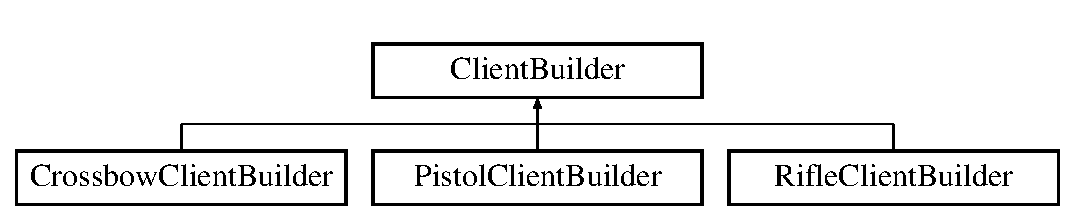
\includegraphics[height=2.000000cm]{classClientBuilder}
\end{center}
\end{figure}
\subsection*{Public Member Functions}
\begin{DoxyCompactItemize}
\item 
void \hyperlink{classClientBuilder_a1a8a43d20d6452aa8f7e55ff7464d4d9}{CreateClient} ()
\item 
\hyperlink{classClient}{Client} $\ast$ \hyperlink{classClientBuilder_a810820bea069cb0612b6a788f290ae11}{RetClient} ()
\item 
virtual void \hyperlink{classClientBuilder_a7c6225251cb997b4cb9d68c77cb67330}{SetBron} ()=0
\end{DoxyCompactItemize}
\subsection*{Protected Attributes}
\begin{DoxyCompactItemize}
\item 
\hyperlink{classClient}{Client} $\ast$ \hyperlink{classClientBuilder_a18ca0906572c5a1a86000c7a51175c23}{itsClient}
\end{DoxyCompactItemize}


\subsection{Detailed Description}
Builder klas Klientow \begin{DoxyAuthor}{Author}
Marcin Fabrykowski 
\end{DoxyAuthor}


\subsection{Member Function Documentation}
\hypertarget{classClientBuilder_a1a8a43d20d6452aa8f7e55ff7464d4d9}{
\index{ClientBuilder@{ClientBuilder}!CreateClient@{CreateClient}}
\index{CreateClient@{CreateClient}!ClientBuilder@{ClientBuilder}}
\subsubsection[{CreateClient}]{\setlength{\rightskip}{0pt plus 5cm}void ClientBuilder::CreateClient (
\begin{DoxyParamCaption}
{}
\end{DoxyParamCaption}
)}}
\label{classClientBuilder_a1a8a43d20d6452aa8f7e55ff7464d4d9}
Tworzenie klienta \hypertarget{classClientBuilder_a810820bea069cb0612b6a788f290ae11}{
\index{ClientBuilder@{ClientBuilder}!RetClient@{RetClient}}
\index{RetClient@{RetClient}!ClientBuilder@{ClientBuilder}}
\subsubsection[{RetClient}]{\setlength{\rightskip}{0pt plus 5cm}{\bf Client}$\ast$ ClientBuilder::RetClient (
\begin{DoxyParamCaption}
{}
\end{DoxyParamCaption}
)\hspace{0.3cm}{\ttfamily  \mbox{[}inline\mbox{]}}}}
\label{classClientBuilder_a810820bea069cb0612b6a788f290ae11}
Zwraca stworzonego klienta \begin{DoxyReturn}{Returns}
Wskaznik do utworzonego klienta 
\end{DoxyReturn}
\hypertarget{classClientBuilder_a7c6225251cb997b4cb9d68c77cb67330}{
\index{ClientBuilder@{ClientBuilder}!SetBron@{SetBron}}
\index{SetBron@{SetBron}!ClientBuilder@{ClientBuilder}}
\subsubsection[{SetBron}]{\setlength{\rightskip}{0pt plus 5cm}virtual void ClientBuilder::SetBron (
\begin{DoxyParamCaption}
{}
\end{DoxyParamCaption}
)\hspace{0.3cm}{\ttfamily  \mbox{[}pure virtual\mbox{]}}}}
\label{classClientBuilder_a7c6225251cb997b4cb9d68c77cb67330}
Wirtualna funkcja ustawiania broni 

Implemented in \hyperlink{classPistolClientBuilder_a74f10c9d757f56e3cc1ae6257a09fea6}{PistolClientBuilder}, \hyperlink{classCrossbowClientBuilder_a1ed4ca8da04961a163aca90d4f7978ee}{CrossbowClientBuilder}, and \hyperlink{classRifleClientBuilder_a65d74c8413cd74184e974b3457d7aaea}{RifleClientBuilder}.



\subsection{Member Data Documentation}
\hypertarget{classClientBuilder_a18ca0906572c5a1a86000c7a51175c23}{
\index{ClientBuilder@{ClientBuilder}!itsClient@{itsClient}}
\index{itsClient@{itsClient}!ClientBuilder@{ClientBuilder}}
\subsubsection[{itsClient}]{\setlength{\rightskip}{0pt plus 5cm}{\bf Client}$\ast$ {\bf ClientBuilder::itsClient}\hspace{0.3cm}{\ttfamily  \mbox{[}protected\mbox{]}}}}
\label{classClientBuilder_a18ca0906572c5a1a86000c7a51175c23}
Wstaznik na utworzonego klienta 

The documentation for this class was generated from the following files:\begin{DoxyCompactItemize}
\item 
client.h\item 
client.cpp\end{DoxyCompactItemize}

\hypertarget{classCrossbowClientBuilder}{
\section{CrossbowClientBuilder Class Reference}
\label{classCrossbowClientBuilder}\index{CrossbowClientBuilder@{CrossbowClientBuilder}}
}


{\ttfamily \#include $<$client.h$>$}

Inheritance diagram for CrossbowClientBuilder:\begin{figure}[H]
\begin{center}
\leavevmode
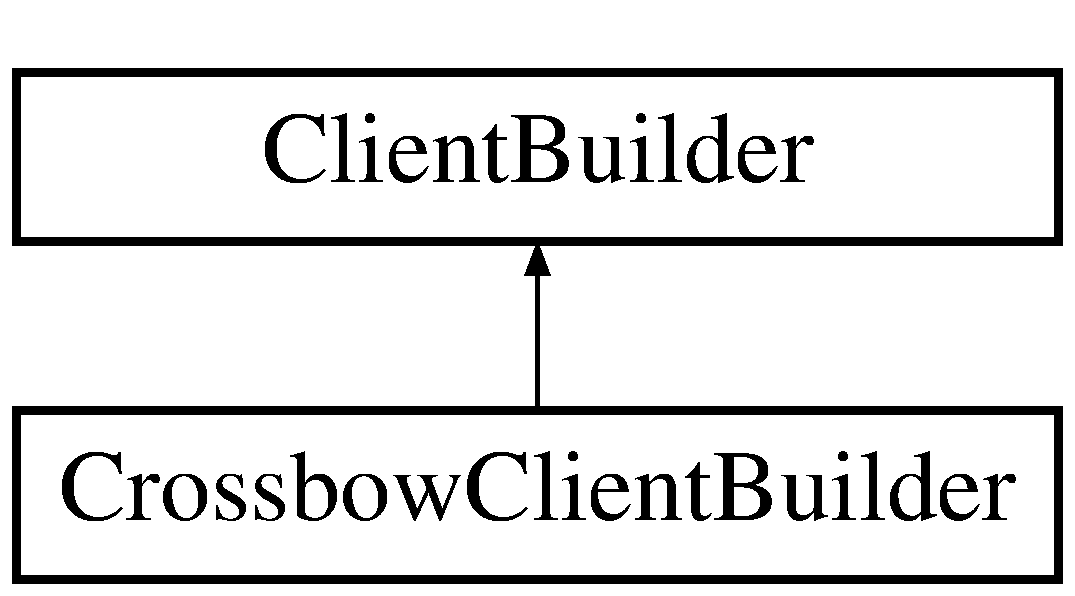
\includegraphics[height=2.000000cm]{classCrossbowClientBuilder}
\end{center}
\end{figure}
\subsection*{Public Member Functions}
\begin{DoxyCompactItemize}
\item 
void \hyperlink{classCrossbowClientBuilder_a1ed4ca8da04961a163aca90d4f7978ee}{SetBron} ()
\end{DoxyCompactItemize}


\subsection{Detailed Description}
Budowniczy Klienta z kusza \begin{DoxyAuthor}{Author}
Marcin Fabrykowski 
\end{DoxyAuthor}


\subsection{Member Function Documentation}
\hypertarget{classCrossbowClientBuilder_a1ed4ca8da04961a163aca90d4f7978ee}{
\index{CrossbowClientBuilder@{CrossbowClientBuilder}!SetBron@{SetBron}}
\index{SetBron@{SetBron}!CrossbowClientBuilder@{CrossbowClientBuilder}}
\subsubsection[{SetBron}]{\setlength{\rightskip}{0pt plus 5cm}void CrossbowClientBuilder::SetBron (
\begin{DoxyParamCaption}
{}
\end{DoxyParamCaption}
)\hspace{0.3cm}{\ttfamily  \mbox{[}virtual\mbox{]}}}}
\label{classCrossbowClientBuilder_a1ed4ca8da04961a163aca90d4f7978ee}
Ustawia kusze jako bron klienta 

Implements \hyperlink{classClientBuilder_a7c6225251cb997b4cb9d68c77cb67330}{ClientBuilder}.



The documentation for this class was generated from the following files:\begin{DoxyCompactItemize}
\item 
client.h\item 
client.cpp\end{DoxyCompactItemize}

\hypertarget{classKaziu}{
\section{Kaziu Class Reference}
\label{classKaziu}\index{Kaziu@{Kaziu}}
}


{\ttfamily \#include $<$kaziu.h$>$}

\subsection*{Public Member Functions}
\begin{DoxyCompactItemize}
\item 
\hyperlink{classClient}{Client} $\ast$ \hyperlink{classKaziu_a360e93daf6fbe5e467c4753dcb666e9b}{Obsluz} ()
\end{DoxyCompactItemize}


\subsection{Detailed Description}
Klasa Pana kazia, obslugujacego klientow \begin{DoxyAuthor}{Author}
Marcin Fabrykowski 
\end{DoxyAuthor}


\subsection{Member Function Documentation}
\hypertarget{classKaziu_a360e93daf6fbe5e467c4753dcb666e9b}{
\index{Kaziu@{Kaziu}!Obsluz@{Obsluz}}
\index{Obsluz@{Obsluz}!Kaziu@{Kaziu}}
\subsubsection[{Obsluz}]{\setlength{\rightskip}{0pt plus 5cm}{\bf Client} $\ast$ Kaziu::Obsluz (
\begin{DoxyParamCaption}
{}
\end{DoxyParamCaption}
)}}
\label{classKaziu_a360e93daf6fbe5e467c4753dcb666e9b}
Obsluguje interesanta, tworzac z niego klienta \begin{DoxyReturn}{Returns}
Wskaznik do nowego klienta 
\end{DoxyReturn}


The documentation for this class was generated from the following files:\begin{DoxyCompactItemize}
\item 
kaziu.h\item 
kaziu.cpp\end{DoxyCompactItemize}

\hypertarget{classLogger}{
\section{Logger Class Reference}
\label{classLogger}\index{Logger@{Logger}}
}


{\ttfamily \#include $<$logger.h$>$}

\subsection*{Public Member Functions}
\begin{DoxyCompactItemize}
\item 
void \hyperlink{classLogger_a82870c41423ead8d99e43ad7f65801c9}{SetPath} (std::string path)
\item 
void \hyperlink{classLogger_a3d5ca95baed18bb70cac5810dd75b078}{StartTimer} ()
\item 
void \hyperlink{classLogger_a1072e97828310d0ea96359b1f2860344}{Log} (std::string data)
\end{DoxyCompactItemize}
\subsection*{Static Public Member Functions}
\begin{DoxyCompactItemize}
\item 
static \hyperlink{classLogger}{Logger} $\ast$ \hyperlink{classLogger_ab01142bf10138e73356980ad146e95ba}{GetInstance} ()
\end{DoxyCompactItemize}


\subsection{Detailed Description}
Klasa logujaca wydarzenia w strzelnicy \begin{DoxyAuthor}{Author}
Marcin Fabrykowski 
\end{DoxyAuthor}


\subsection{Member Function Documentation}
\hypertarget{classLogger_ab01142bf10138e73356980ad146e95ba}{
\index{Logger@{Logger}!GetInstance@{GetInstance}}
\index{GetInstance@{GetInstance}!Logger@{Logger}}
\subsubsection[{GetInstance}]{\setlength{\rightskip}{0pt plus 5cm}static {\bf Logger}$\ast$ Logger::GetInstance (
\begin{DoxyParamCaption}
{}
\end{DoxyParamCaption}
)\hspace{0.3cm}{\ttfamily  \mbox{[}inline, static\mbox{]}}}}
\label{classLogger_ab01142bf10138e73356980ad146e95ba}
Zwraca instancje singletona \begin{DoxyReturn}{Returns}
Wskaznik na jedyna instancje 
\end{DoxyReturn}
\hypertarget{classLogger_a1072e97828310d0ea96359b1f2860344}{
\index{Logger@{Logger}!Log@{Log}}
\index{Log@{Log}!Logger@{Logger}}
\subsubsection[{Log}]{\setlength{\rightskip}{0pt plus 5cm}void Logger::Log (
\begin{DoxyParamCaption}
\item[{std::string}]{data}
\end{DoxyParamCaption}
)}}
\label{classLogger_a1072e97828310d0ea96359b1f2860344}
Loguje zadany ciag znakow. Automatycznie dodaje znak konca lini 
\begin{DoxyParams}{Parameters}
{\em data} & Dane do zalogowania \\
\hline
\end{DoxyParams}
\hypertarget{classLogger_a82870c41423ead8d99e43ad7f65801c9}{
\index{Logger@{Logger}!SetPath@{SetPath}}
\index{SetPath@{SetPath}!Logger@{Logger}}
\subsubsection[{SetPath}]{\setlength{\rightskip}{0pt plus 5cm}void Logger::SetPath (
\begin{DoxyParamCaption}
\item[{std::string}]{path}
\end{DoxyParamCaption}
)\hspace{0.3cm}{\ttfamily  \mbox{[}inline\mbox{]}}}}
\label{classLogger_a82870c41423ead8d99e43ad7f65801c9}
Ustawia sciezke do pliku logow. Jesli plik istnieje, zostanie nadpisany 
\begin{DoxyParams}{Parameters}
{\em path} & sciezka do pliku \\
\hline
\end{DoxyParams}
\hypertarget{classLogger_a3d5ca95baed18bb70cac5810dd75b078}{
\index{Logger@{Logger}!StartTimer@{StartTimer}}
\index{StartTimer@{StartTimer}!Logger@{Logger}}
\subsubsection[{StartTimer}]{\setlength{\rightskip}{0pt plus 5cm}void Logger::StartTimer (
\begin{DoxyParamCaption}
{}
\end{DoxyParamCaption}
)\hspace{0.3cm}{\ttfamily  \mbox{[}inline\mbox{]}}}}
\label{classLogger_a3d5ca95baed18bb70cac5810dd75b078}
Ustawia moemnt od ktorego bedzie liczony czas w logach 

The documentation for this class was generated from the following files:\begin{DoxyCompactItemize}
\item 
logger.h\item 
logger.cpp\end{DoxyCompactItemize}

\hypertarget{classPistolClientBuilder}{
\section{PistolClientBuilder Class Reference}
\label{classPistolClientBuilder}\index{PistolClientBuilder@{PistolClientBuilder}}
}


{\ttfamily \#include $<$client.h$>$}

Inheritance diagram for PistolClientBuilder:\begin{figure}[H]
\begin{center}
\leavevmode
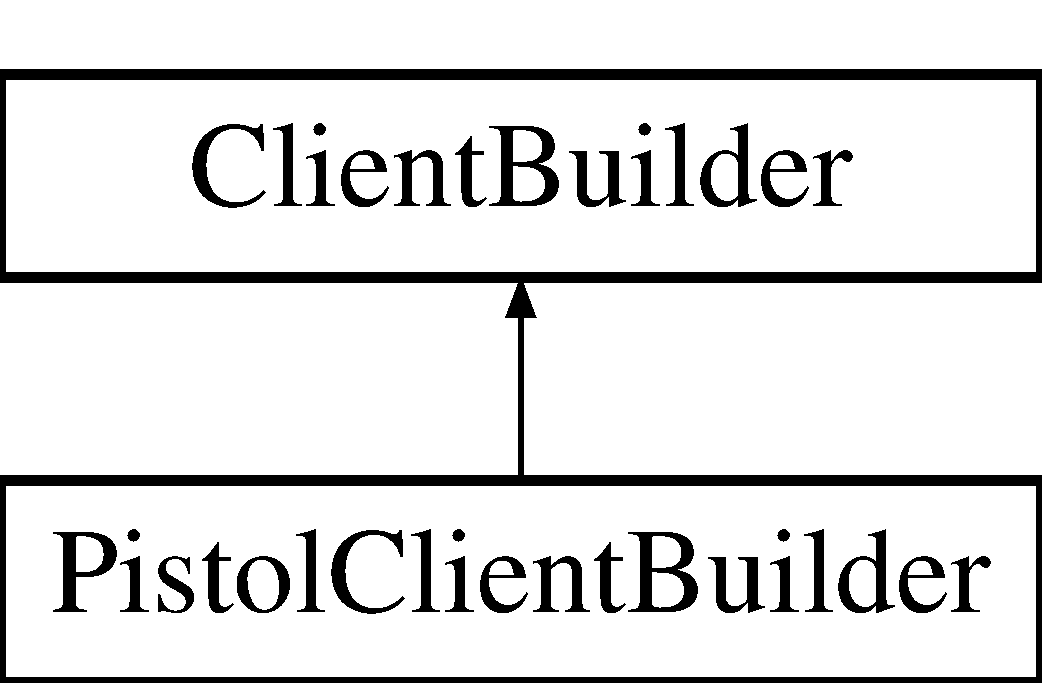
\includegraphics[height=2.000000cm]{classPistolClientBuilder}
\end{center}
\end{figure}
\subsection*{Public Member Functions}
\begin{DoxyCompactItemize}
\item 
void \hyperlink{classPistolClientBuilder_a74f10c9d757f56e3cc1ae6257a09fea6}{SetBron} ()
\end{DoxyCompactItemize}


\subsection{Detailed Description}
Budowniczy Klienta z pistoletem \begin{DoxyAuthor}{Author}
Marcin Fabrykowski 
\end{DoxyAuthor}


\subsection{Member Function Documentation}
\hypertarget{classPistolClientBuilder_a74f10c9d757f56e3cc1ae6257a09fea6}{
\index{PistolClientBuilder@{PistolClientBuilder}!SetBron@{SetBron}}
\index{SetBron@{SetBron}!PistolClientBuilder@{PistolClientBuilder}}
\subsubsection[{SetBron}]{\setlength{\rightskip}{0pt plus 5cm}void PistolClientBuilder::SetBron (
\begin{DoxyParamCaption}
{}
\end{DoxyParamCaption}
)\hspace{0.3cm}{\ttfamily  \mbox{[}virtual\mbox{]}}}}
\label{classPistolClientBuilder_a74f10c9d757f56e3cc1ae6257a09fea6}
Ustawia pistolet jako bron klienta 

Implements \hyperlink{classClientBuilder_a7c6225251cb997b4cb9d68c77cb67330}{ClientBuilder}.



The documentation for this class was generated from the following files:\begin{DoxyCompactItemize}
\item 
client.h\item 
client.cpp\end{DoxyCompactItemize}

\hypertarget{classRifleClientBuilder}{
\section{RifleClientBuilder Class Reference}
\label{classRifleClientBuilder}\index{RifleClientBuilder@{RifleClientBuilder}}
}


{\ttfamily \#include $<$client.h$>$}

Inheritance diagram for RifleClientBuilder:\begin{figure}[H]
\begin{center}
\leavevmode
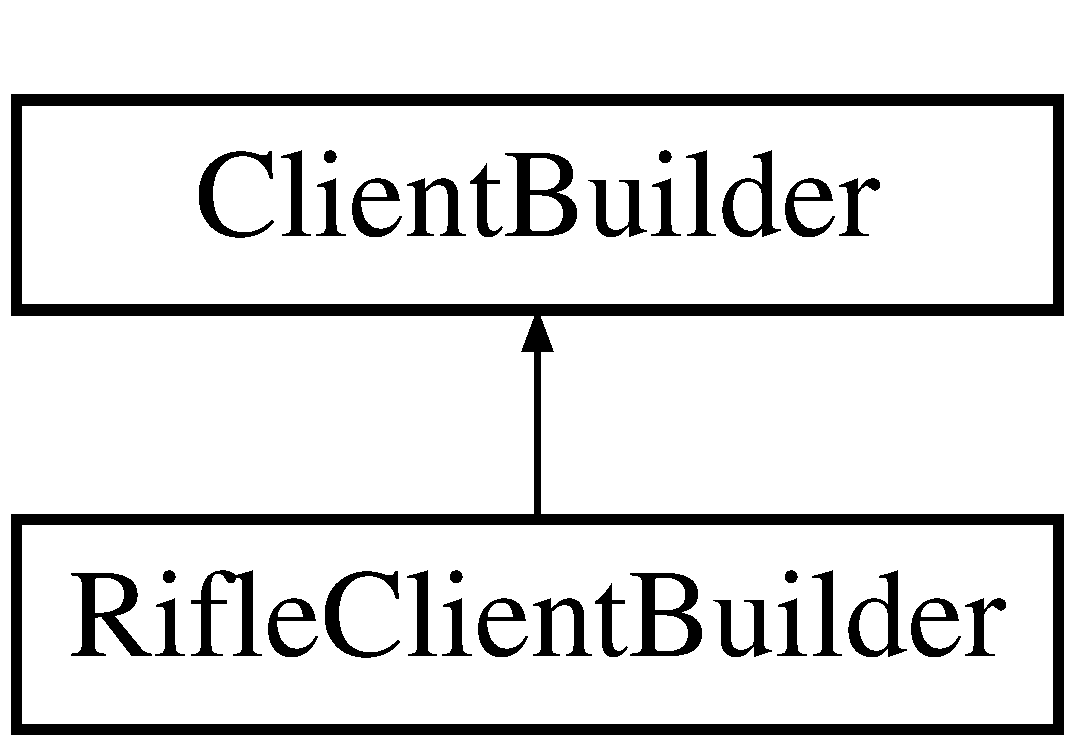
\includegraphics[height=2.000000cm]{classRifleClientBuilder}
\end{center}
\end{figure}
\subsection*{Public Member Functions}
\begin{DoxyCompactItemize}
\item 
void \hyperlink{classRifleClientBuilder_a65d74c8413cd74184e974b3457d7aaea}{SetBron} ()
\end{DoxyCompactItemize}


\subsection{Detailed Description}
Budowniczy Klienta z karabinem \begin{DoxyAuthor}{Author}
Marcin Fabrykowski 
\end{DoxyAuthor}


\subsection{Member Function Documentation}
\hypertarget{classRifleClientBuilder_a65d74c8413cd74184e974b3457d7aaea}{
\index{RifleClientBuilder@{RifleClientBuilder}!SetBron@{SetBron}}
\index{SetBron@{SetBron}!RifleClientBuilder@{RifleClientBuilder}}
\subsubsection[{SetBron}]{\setlength{\rightskip}{0pt plus 5cm}void RifleClientBuilder::SetBron (
\begin{DoxyParamCaption}
{}
\end{DoxyParamCaption}
)\hspace{0.3cm}{\ttfamily  \mbox{[}virtual\mbox{]}}}}
\label{classRifleClientBuilder_a65d74c8413cd74184e974b3457d7aaea}
Ustawia karabin jako bron 

Implements \hyperlink{classClientBuilder_a7c6225251cb997b4cb9d68c77cb67330}{ClientBuilder}.



The documentation for this class was generated from the following files:\begin{DoxyCompactItemize}
\item 
client.h\item 
client.cpp\end{DoxyCompactItemize}

\hypertarget{classStrzelnica}{
\section{Strzelnica Class Reference}
\label{classStrzelnica}\index{Strzelnica@{Strzelnica}}
}


{\ttfamily \#include $<$strzelnica.h$>$}

\subsection*{Public Member Functions}
\begin{DoxyCompactItemize}
\item 
void \hyperlink{classStrzelnica_a302cebea01b16fab0af5d3f59cac9711}{Nowy} ()
\item 
void \hyperlink{classStrzelnica_ad79a2e13f258397bec5a1a4f9957950a}{Zamknij} ()
\item 
pthread\_\-t \hyperlink{classStrzelnica_a87418d047f58586ba4b597a976a0dd3f}{RetMainLoopThread} ()
\end{DoxyCompactItemize}
\subsection*{Static Public Member Functions}
\begin{DoxyCompactItemize}
\item 
static \hyperlink{classStrzelnica}{Strzelnica} $\ast$ \hyperlink{classStrzelnica_a29520cd8701e353e057114b9c00910ca}{GetInstance} ()
\item 
static void $\ast$ \hyperlink{classStrzelnica_a607aab055cd7b761fe5221d25f910c03}{MainLoop} (void $\ast$ptr)
\end{DoxyCompactItemize}


\subsection{Detailed Description}
Klasa zajmujaca sie obsluga strzelnicy \begin{DoxyAuthor}{Author}
Marcin Fabrykowski 
\end{DoxyAuthor}


\subsection{Member Function Documentation}
\hypertarget{classStrzelnica_a29520cd8701e353e057114b9c00910ca}{
\index{Strzelnica@{Strzelnica}!GetInstance@{GetInstance}}
\index{GetInstance@{GetInstance}!Strzelnica@{Strzelnica}}
\subsubsection[{GetInstance}]{\setlength{\rightskip}{0pt plus 5cm}static {\bf Strzelnica}$\ast$ Strzelnica::GetInstance (
\begin{DoxyParamCaption}
{}
\end{DoxyParamCaption}
)\hspace{0.3cm}{\ttfamily  \mbox{[}inline, static\mbox{]}}}}
\label{classStrzelnica_a29520cd8701e353e057114b9c00910ca}
Zwraca wskaznik na instancje singletona \begin{DoxyReturn}{Returns}
Wskaznik na instancje Strzelnicy 
\end{DoxyReturn}
\hypertarget{classStrzelnica_a607aab055cd7b761fe5221d25f910c03}{
\index{Strzelnica@{Strzelnica}!MainLoop@{MainLoop}}
\index{MainLoop@{MainLoop}!Strzelnica@{Strzelnica}}
\subsubsection[{MainLoop}]{\setlength{\rightskip}{0pt plus 5cm}void $\ast$ Strzelnica::MainLoop (
\begin{DoxyParamCaption}
\item[{void $\ast$}]{ptr}
\end{DoxyParamCaption}
)\hspace{0.3cm}{\ttfamily  \mbox{[}static\mbox{]}}}}
\label{classStrzelnica_a607aab055cd7b761fe5221d25f910c03}
Glowna petla pobierajaca klientow z kolejki i umieszczajaca ich na odpowiednich torach 
\begin{DoxyParams}{Parameters}
{\em ptr} & nieuzywane \\
\hline
\end{DoxyParams}
\hypertarget{classStrzelnica_a302cebea01b16fab0af5d3f59cac9711}{
\index{Strzelnica@{Strzelnica}!Nowy@{Nowy}}
\index{Nowy@{Nowy}!Strzelnica@{Strzelnica}}
\subsubsection[{Nowy}]{\setlength{\rightskip}{0pt plus 5cm}void Strzelnica::Nowy (
\begin{DoxyParamCaption}
{}
\end{DoxyParamCaption}
)}}
\label{classStrzelnica_a302cebea01b16fab0af5d3f59cac9711}
Symuluje nowego interesanta \hypertarget{classStrzelnica_a87418d047f58586ba4b597a976a0dd3f}{
\index{Strzelnica@{Strzelnica}!RetMainLoopThread@{RetMainLoopThread}}
\index{RetMainLoopThread@{RetMainLoopThread}!Strzelnica@{Strzelnica}}
\subsubsection[{RetMainLoopThread}]{\setlength{\rightskip}{0pt plus 5cm}pthread\_\-t Strzelnica::RetMainLoopThread (
\begin{DoxyParamCaption}
{}
\end{DoxyParamCaption}
)\hspace{0.3cm}{\ttfamily  \mbox{[}inline\mbox{]}}}}
\label{classStrzelnica_a87418d047f58586ba4b597a976a0dd3f}
Zwraca id watku glowej petli strzelnicy \begin{DoxyReturn}{Returns}
id watku MainLoop 
\end{DoxyReturn}
\hypertarget{classStrzelnica_ad79a2e13f258397bec5a1a4f9957950a}{
\index{Strzelnica@{Strzelnica}!Zamknij@{Zamknij}}
\index{Zamknij@{Zamknij}!Strzelnica@{Strzelnica}}
\subsubsection[{Zamknij}]{\setlength{\rightskip}{0pt plus 5cm}void Strzelnica::Zamknij (
\begin{DoxyParamCaption}
{}
\end{DoxyParamCaption}
)\hspace{0.3cm}{\ttfamily  \mbox{[}inline\mbox{]}}}}
\label{classStrzelnica_ad79a2e13f258397bec5a1a4f9957950a}
Zamyka strzelnice. Oczekuje do skonczenia strzelania klientow w strzelnicy 

The documentation for this class was generated from the following files:\begin{DoxyCompactItemize}
\item 
strzelnica.h\item 
strzelnica.cpp\end{DoxyCompactItemize}

\printindex
\end{document}
